\documentclass[12pt, a4paper]{article}

% ── Packages ──────────────────────────────────────────────────────────────────
\usepackage{amsmath, amssymb, amsthm}
\usepackage{geometry}
\usepackage{booktabs}
\usepackage{array}
\usepackage{hyperref}
\usepackage{xcolor}
\usepackage{tcolorbox}
\usepackage{enumitem}
\usepackage{parskip}
\usepackage{tikz}
\usetikzlibrary{arrows.meta, positioning, calc}

\geometry{margin=2.5cm}

% ── Student-mode switch ───────────────────────────────────────────────────────
\newif\ifstudentmode
\studentmodefalse
\ifx\studentflag\undefined\else\studentmodetrue\fi

\newcommand{\sol}[2][6cm]{%
  \ifstudentmode\underline{\hspace{#1}}\else{#2}\fi}

\newcommand{\soleq}[2][3cm]{%
  \ifstudentmode
    \par\vspace{4pt}\noindent\rule{\linewidth}{0.5pt}\\[#1]%
    \noindent\rule{\linewidth}{0.5pt}\par\vspace{4pt}%
  \else\[#2\]\fi}

% ── Colors & boxes ────────────────────────────────────────────────────────────
\definecolor{mainblue}{RGB}{30, 100, 180}
\definecolor{boxbg}{RGB}{235, 243, 255}
\definecolor{notebg}{RGB}{255, 248, 230}
\definecolor{warnbg}{RGB}{255, 235, 235}
\definecolor{greenbg}{RGB}{230, 255, 235}

\tcbuselibrary{skins, breakable}

\newtcolorbox{resultbox}{colback=boxbg,colframe=mainblue,boxrule=1.2pt,arc=4pt,
  title={Result},fonttitle=\bfseries\color{white},coltitle=white,
  attach boxed title to top left={yshift=-2mm,xshift=4mm},
  boxed title style={colback=mainblue,arc=3pt}}

\newtcolorbox{notebox}{colback=notebg,colframe=orange!70!black,
  boxrule=1pt,arc=4pt,left=4pt,right=4pt}

\newtcolorbox{warnbox}{colback=warnbg,colframe=red!60!black,
  boxrule=1pt,arc=4pt,left=4pt,right=4pt}

\newtcolorbox{stepbox}[1]{colback=greenbg,colframe=green!50!black,
  boxrule=1pt,arc=4pt,title={#1},fonttitle=\bfseries,coltitle=green!30!black}

\theoremstyle{definition}
\newtheorem{example}{Example}[section]

\newcommand{\yhat}{\hat{y}}
\newcommand{\norm}[1]{\left\|#1\right\|}

% ── Document ──────────────────────────────────────────────────────────────────
\begin{document}

\begin{center}
  {\LARGE \textbf{Section 4.1: Regularization}} \\[0.3em]
  {\large\itshape L1 and L2 — Teaching the Network to Generalise} \\[0.5em]
  {\large AI Class --- Lecture Notes}%
  \ifstudentmode\quad{\normalsize\color{gray}[Student Copy]}\fi
\end{center}

\vspace{1em}\hrule\vspace{1.5em}

% ══════════════════════════════════════════════════════════════════════════════
\section{The Problem: Overfitting}

A network trained long enough on a small dataset will eventually
\textbf{memorise} the training examples rather than learning the underlying
pattern.  It achieves near-zero training loss but fails badly on new data.

\begin{center}
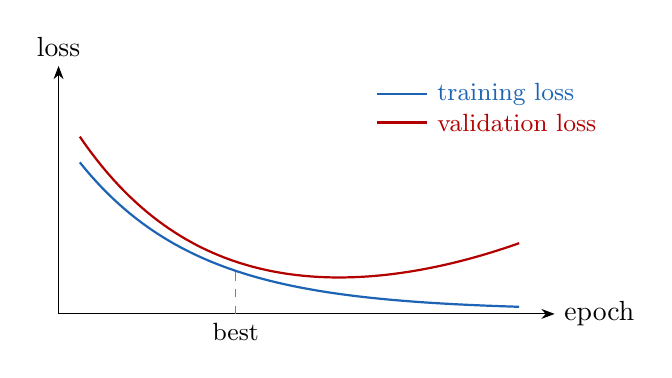
\begin{tikzpicture}[scale=0.9, >=Stealth]
  \draw[->] (0,0) -- (7,0) node[right] {epoch};
  \draw[->] (0,0) -- (0,3.5) node[above] {loss};
  % Training loss curve (decreasing)
  \draw[thick, mainblue, domain=0.3:6.5, samples=80]
    plot (\x, {2.5*exp(-0.6*\x) + 0.05});
  % Validation loss curve (U-shaped)
  \draw[thick, red!70!black, domain=0.3:6.5, samples=80]
    plot (\x, {2.5*exp(-0.6*\x) + 0.4*(\x-2.5)^2*0.12 + 0.18});
  % Best point marker
  \draw[dashed, gray] (2.5,0) -- (2.5,0.7);
  \node[below] at (2.5,0) {\small best};
  % Legend
  \draw[thick, mainblue] (4.5,3.1) -- (5.2,3.1)
    node[right, font=\small] {training loss};
  \draw[thick, red!70!black] (4.5,2.7) -- (5.2,2.7)
    node[right, font=\small] {validation loss};
\end{tikzpicture}
\end{center}

The validation loss initially decreases together with the training loss,
then starts rising --- the network is now fitting noise.
\textbf{Regularisation} discourages this by penalising large weights,
which are the symptom of overfitting.

% ══════════════════════════════════════════════════════════════════════════════
\section{L2 Regularisation (Weight Decay)}

Add the sum of squared weights to the loss:

\begin{resultbox}
\[
  J_{\text{reg}} = J + \lambda \sum_i w_i^2
\]
where $\lambda > 0$ controls how strongly large weights are penalised.
\end{resultbox}

\subsection{Effect on the Gradient}

Taking the partial derivative:
\[
  \frac{\partial J_{\text{reg}}}{\partial w}
  = \frac{\partial J}{\partial w} + \sol[3cm]{2\lambda w}
\]

The gradient descent update becomes:
\[
  w \;\longleftarrow\; w - \eta\!\left(\frac{\partial J}{\partial w} + 2\lambda w\right)
\]

Rearranging:
\[
  w \;\longleftarrow\; \underbrace{(1 - 2\eta\lambda)}_{\text{shrink factor}}\, w
                    \;-\; \eta\,\frac{\partial J}{\partial w}
\]

Every update \emph{shrinks} the weight slightly toward zero before applying
the gradient step.  This is why L2 regularisation is also called
\textbf{weight decay}.

\subsection{Hand-Calculated Example}

Using $w^{(2)}_1 = 0.5$, gradient $g = -0.084$ (from Section 3.4),
$\eta = 0.1$, and $\lambda = 0.01$:

\begin{stepbox}{Without regularisation}
\[
  w \leftarrow 0.5 - 0.1 \times (-0.084) = \sol[4cm]{0.5084}
\]
\end{stepbox}

\vspace{0.6em}

\begin{stepbox}{With L2 regularisation}
\[
  \frac{\partial J_{\text{reg}}}{\partial w}
  = -0.084 + 2(0.01)(0.5) = -0.084 + 0.010 = \sol[3cm]{-0.074}
\]
\[
  w \leftarrow 0.5 - 0.1 \times (-0.074) = \sol[4cm]{0.5074}
\]
\end{stepbox}

\vspace{0.4em}

The regularised update is slightly smaller ($0.5074$ vs $0.5084$): the
penalty pulled the weight back toward zero by $0.001$.  Small per step, but
it accumulates over thousands of updates.

% ══════════════════════════════════════════════════════════════════════════════
\section{L1 Regularisation (Sparsity)}

Replace the squared penalty with the \emph{absolute value}:

\begin{resultbox}
\[
  J_{\text{reg}} = J + \lambda \sum_i |w_i|
\]
\end{resultbox}

\subsection{Effect on the Gradient}

\[
  \frac{\partial J_{\text{reg}}}{\partial w}
  = \frac{\partial J}{\partial w} + \sol[4cm]{\lambda\,\operatorname{sign}(w)}
\]

where $\operatorname{sign}(w) = +1$ if $w > 0$, and $-1$ if $w < 0$.

Unlike L2, the penalty is \textbf{constant} --- it does not scale with $|w|$.
This means L1 applies the same pressure to a weight of $0.5$ as to a weight
of $0.001$, and will push even tiny weights all the way to zero.

\subsection{L1 vs L2: The Key Difference}

The distinction shows up clearly when comparing a large weight and a small
weight under the same conditions ($g = -0.084$, $\lambda = 0.01$):

\begin{center}
\renewcommand{\arraystretch}{1.6}
\begin{tabular}{llcc}
\toprule
Weight & Method & $\partial J_{\text{reg}}/\partial w$ & $w_{\text{new}}$ ($\eta=0.1$) \\
\midrule
$w = 0.5$ & No reg       & $-0.084$                              & $0.508$ \\
           & L2           & $-0.084 + 2(0.01)(0.5) = -0.074$     & $0.507$ \\
           & L1           & $-0.084 + 0.01(+1) = -0.074$         & $0.507$ \\
\midrule
$w = 0.01$ & No reg      & $-0.084$                              & $0.018$ \\
            & L2          & $-0.084 + 2(0.01)(0.01) = -0.0838$   & $0.019$ \\
            & L1          & $-0.084 + 0.01(+1) = -0.074$         & $0.017$ \\
\bottomrule
\end{tabular}
\end{center}

For the large weight ($w=0.5$), L1 and L2 give almost identical results.
For the small weight ($w=0.01$), L2 barely penalises it (penalty $= 0.0002$)
while L1 applies full pressure (penalty $= 0.01$) --- driving it toward zero.

\begin{notebox}
\textbf{When to use which:}
Use \textbf{L2} when you expect many small weights to all contribute.
Use \textbf{L1} when you expect only a few weights to matter and want the
rest to vanish completely (sparse solution).
In practice L2 is the default; L1 is common in feature selection.
\end{notebox}

% ══════════════════════════════════════════════════════════════════════════════
\section{Choosing $\lambda$}

\begin{center}
\renewcommand{\arraystretch}{1.3}
\begin{tabular}{lll}
\toprule
$\lambda$ & Effect & Symptom \\
\midrule
Too small & Almost no regularisation & Validation loss diverges from training loss \\
Good      & Validation loss tracks training loss & Model generalises well \\
Too large & Weights shrink to near zero & Both training and validation loss stay high \\
\bottomrule
\end{tabular}
\end{center}

Typical starting values: $\lambda \in \{10^{-4}, 10^{-3}, 10^{-2}\}$.
Tune by monitoring the gap between training and validation loss.

\begin{notebox}
\textbf{PyTorch.}
L2 regularisation is built into every PyTorch optimiser as
\texttt{weight\_decay}.  See \texttt{code\_examples.py} for usage.
L1 is added manually to the loss; an example is also in the code file.
\end{notebox}

\end{document}
